\documentclass{article}
\usepackage[utf8]{inputenc} % UTF-8
\usepackage{amsmath}
\usepackage{amssymb}
\usepackage{algpseudocode} % Algoritmos
\usepackage[a4paper, total={6in, 8in}]{geometry}
\usepackage{graphicx} % Figuras e imagenes
\usepackage{multirow} % Combinacion de celdas en tablas
\usepackage{algorithmicx}
\usepackage{fancyhdr} % Cabeceras y pies de pagina
\usepackage{blindtext} % lorem ipsum dolor...
\graphicspath{ {images/} } % Ruta a las imagenes

\title{Práctica 2 - Problemas de optimización con técnicas basadas en poblaciones}
\author{Luis Miguel Guirado Bautista}
\date{20 de Mayo de 2022 \qquad Curso 2021/2022}

\pagestyle{fancy}
\fancyhf{}

% do-while en algoritmos
\algdef{SE}[DOWHILE]{Do}{doWhile}{\algorithmicdo}[1]{\algorithmicwhile\ #1}%

\renewcommand*\contentsname{Índice} % Nombre del indice
\renewcommand{\figurename}{Figura} % Nombre de una figura
\renewcommand{\partname}{Ejercicio} % Nombre de \part
\renewcommand{\familydefault}{\sfdefault}

\begin{document}

    \begin{titlepage}
        \maketitle
        \thispagestyle{empty}
        \begin{enumerate}
            \item[\textbf{Correo:}]luismgb@correo.ugr.es
            \item[\textbf{DNI:}]75942712R
            \item[\textbf{Subgrupo:}]Martes, 3
            \item[\textbf{Problema:}]Mínima Dispersión Diferencial 
        \end{enumerate}
    \end{titlepage}

    \pagebreak

    \lhead{Práctica 2 - Metaheurísticas}
    \rhead{Luis Miguel Guirado Bautista}
    \tableofcontents

    \pagebreak
    \rfoot{\thepage}
    \section{Motivación}

    En esta práctica abordaremos el problema de la Mínima Dispersión Diferencial, que
    consiste en seleccionar un subconjunto de puntos ya definidos en el plano tal que
    la dispersión entre ellos sea mínima.

    Siendo $i$ y $j$ dos puntos del plano y $S$ el subconjunto de puntos
    seleccionados, la función objetivo (dispersión de los puntos seleccionados) es:

    \begin{equation*}
        \Delta(S) = max_{i \in S}(\sum_{j \in S}{d_{ij}}) - min_{i \in M}(\sum_{j \in S}{d_{ij}})
    \end{equation*}

    Siendo $n$ el número de posibles destinos, la matriz de distancias entre los $n$ puntos
    se define como:

    \begin{equation*}
        D =
        \begin{pmatrix}
            0 & d_{12} & d_{13} & \dots & d_{1n} \\
            d_{21} & 0 & d_{12} & \dots & d_{2n} \\
            d_{31} & d_{32} & 0 & \dots & d_{3n} \\
            \vdots & \vdots & \vdots & \ddots & \vdots \\
            d_{n1} & d_{n2} & d_{n3} & \dots & d_{nn} \\
        \end{pmatrix}
    \end{equation*}

    El fichero \texttt{datos} de la práctica contiene la diagonal superior de 50 matrices
    de distancias.
    
    Consideraremos $D_{b}$ la matriz de distancias del caso $b$.

    Para este problema usaremos los siguientes algortimos:

    \begin{itemize}
        \item Greedy.
        Ir escogiendo los que menor dispersión supongan a partir de un punto aleatorio.
        \item Búsqueda Local.
        A partir de un subconjunto $S$ aleatorio, intercambiar ciertos puntos de $S$ con los
        del resto de puntos de manera que la dispersión entre la solución antigua y la nueva
        se vea reducida.
        \item Algoritmos Genéticos.
        Simular una población de soluciones $P$ y finalmente escoger la mejor solución de
        todo $P$. Utilizaremos dos variantes:
        \begin{itemize}
            \item Generacional.
            \item Estacionario.
        \end{itemize}
        Y cada una de estas variantes tendrá otras subvariantes según el tipo de cruce que se
        vaya a emplear a la hora de realizar la simulación:
        \begin{itemize}
            \item Cruce uniforme. (AGG-Uniforme y AGE-Uniforme)
            \item Cruce de posición. (AGG-Posición y AGE-Posición)
        \end{itemize}
        \item Algoritmo Memético.
        Híbrido entre el AGG-Uniforme y Búsqueda Local. Usaremos tres variantes según la
        probabilidad de que se aplique Búsqueda Local.
        \begin{itemize}
            \item AM(10,1).
            Cada 10 generaciones, se aplica Búsqueda Local en todo $P$.
            \item AM(10,0.1).
            Cada 10 generaciones, se aplica Búsqueda Local en $0.1|P|$ individuos aleatorios.
            \item AM(10,0.1-mej).
            Cada 10 generaciones, se aplica Búsqueda Local en los mejores $0.1|P|$ individuos.
        \end{itemize}
    \end{itemize}

    \paragraph*{Nota}No se ha realizado el AM

    \pagebreak
    \section{Aplicación de los algoritmos al problema}

    Para todos los algoritmos, salvo el memético, representaremos $S$ como un vector
    binario, por ejemplo, si en $S$ tenemos los puntos $\{1,2,4\}$ y $n = 5$:
    \begin{equation*}
        S_{bin} = [1,1,0,1,0]
    \end{equation*}

    \subsection{Greedy}

    Comenzaremos el algoritmo escogiendo un punto aleatorio del plano
    para añadirlo a nuestra solución $S$, e iremos añadiendo más puntos
    a $S$ según el siguiente criterio:

    \begin{equation*}
        u^* = min_{u \notin S}(g(u))
    \end{equation*}

    Es decir, el punto cuya $g(u)$ sea la menor de todas.
    El cálculo de $g(u)$ se hace así:

    \begin{equation*}
        u \notin S;\;\partial(u) = \sum_{v \in S}d_{uv}
    \end{equation*}

    \begin{equation*}
        v \in S;\;\partial(v) = d_{uv} + SumaAnterior(v)
    \end{equation*}

    \paragraph*{Nota}Siendo $v'$ el punto anterior a $v$, $SumaAnterior(v)$ es $\partial(v')$.
    Si es el primer punto de $S$, entonces $SumaAnterior(v) = 0$

    \begin{equation*}
        \partial_{max}(u) = max(\partial(u), max_{v \in S}(\partial(v)))
    \end{equation*}

    \begin{equation*}
        \partial_{min}(u) = min(\partial(u), min_{v \in S}(\partial(v)))
    \end{equation*}

    \begin{equation*}
        g(u) = \partial_{max}(u) - \partial_{min}(u)
    \end{equation*}

    Parará cuando $|S| = m$, entonces devolverá la solución y su dispersión (no $g(u)$).

    \subsection{Búsqueda Local}

    Comienza con una solución completa y aleatoria. Entonces para cada punto $u \in S$ y
    $v \notin S$, se genera una solución $S'$ que resulta de intercambiar el elemento $u$
    con el elemento $v$. Esto se repite hasta que se haya alcanzado el máximo de iteraciones
    $T = 100.000$ o no se haya encontrado una $S'$ que sea mejor que $S$.
    $S'$ reemplazará a $S$ si:

    \begin{equation*}
        \Delta Z_{mm} = Z_{mm}(S') - Z_{mm}(S) < 0
    \end{equation*}
    \begin{equation*}
        Z_{mm}(S') = (\partial_{max}^{'} - \partial_{min}^{'})
    \end{equation*}
    \begin{equation*}
        \partial_{max}^{'} = max(\partial(v), max_{w \in S}(\partial(w)))
    \end{equation*}
    \begin{equation*}
        \partial_{min}^{'} = min(\partial(v), min_{w \in S}(\partial(w)))
    \end{equation*}
    \begin{equation*}
        \partial(v) = \sum_{w \in S}d_{vw}
    \end{equation*}
    \begin{equation*}
        \partial(w) = SumaAnterior(w) - d_{wu} + d_{wv}
    \end{equation*}

    \pagebreak
    \subsection{Genético}

    Los algortimos genéticos consisten en generar un conjunto de soluciones $P$ y
    aplicarles una serie de cómputos hasta que se hayan alcanzado $T$ iteraciones
    (o generaciones), entonces devolverá el mejor individuo de todos 
    y su dispersión (valoraremos por MDD).

    \begin{itemize}
        \item Selección.
        Seleccionamos unos individuos de $P$ para aplicar el siguiente paso.
        \item Cruce.
        Escoger dos individuos y \emph{escoger lo mejor} de cada uno para
        generar otro individuo que será el hijo.
        \item Mutación.
        Modificar ligeramente o no los individuos del conjunto anterior.
        Intercambiaremos un elemento $x_i$ con otro $x_j$ t.q el valor de estos
        no sean iguales.
        \item Reemplazamiento.
        Insertar los hijos en $P$.
    \end{itemize}

    Siendo dos padres $S_1$ y $S_2$ y su hijo $S_h$,
    para cada una de las variantes de los algoritmos genéticos (generacional y
    estacionario), consideraremos otras subvariantes dependiendo del tipo de cruce
    que realizen, que puede ser:

    \begin{itemize}
        \item Uniforme.
        Cada elemento (gen) en común con $S_1$ y $S_2$ los hereda $S_h$. El resto de
        elementos son escogidos aleatoriamente entre los dos padres. Esto da lugar a
        soluciones que no son factibles, por lo que requerirá un \emph{reparador} para
        que vuelvan a ser factibles.
        \item De posición.
        Este es más simple, cada elemento de la solución en común con $S_1$ y $S_2$
        los hereda $S_h$ como en el anterior. Pero ahora los genes restantes se escogen
        de un padre y se le asignan aleatoriamente a $S_h$
    \end{itemize}

    \subsubsection{Generacional}

    \begin{itemize}
        \item Selección.
        Seleccionamos todos los individuos de $P$. De modo que $P = P'$
        \item Cruce.
        Siendo $p_c = 0.7$ la probabilidad de cruce, cruzaremos las primeras
        $\left\lfloor\frac{|P|}{2}\cdot p_c\right\rfloor$ parejas.
        \item Mutación.
        Siendo $p_m = 0.1$ la probabilidad de mutación, mutaremos
        $\left\lfloor|P|\cdot p_m\right\rfloor$ veces a los individuos de $P'$
        de forma aleatoria, además, un individuo podrá mutar varias veces por
        iteración.
        \item Reemplazamiento.
        Si el mejor individuo de $P$ no sobrevive,
        entonces reemplazaremos el peor individuo de $P'$ por el
        mejor de $P$.
    \end{itemize}

    \subsubsection{Estacionario}

    \begin{itemize}
        \item Selección.
        Seleccionamos dos padres $S_1$ y $S_2$ mediante torneo binario,
        entonces $P' = \{S_1, S_2\}$
        \item Cruce.
        Se cruzan $P'$ dos veces, y sus hijos reemplazan a los padres.
        \item Mutación.
        Siendo $p_m = 0.1$ la probabilidad de mutación, generaremos un
        número aleatorio $r \in [0,1]$ para cada uno de los hijos,
        si $r < p_m$ entonces ese hijo mutará
        \item Reemplazamiento.
        Los hijos compiten para ver quien entra a $P$, el ganador
        reemplazará al peor individuo de $P$.
    \end{itemize}

    \pagebreak
    \section{Algoritmos empleados (pseudocódigo)}

    \subsection{Greedy}

    \begin{algorithmic}
        \Function{EscogerGreedy}{$D$, $S$}
            \State{$sumas \gets 0_{n}$} \Comment{Vector de $n$ ceros.}
            \State{$mejor\_disp \gets \infty$}
            \State{$mejor \gets$ \texttt{RandomChoice}$([0,n))$} \Comment{Función de NumPy. Entero aleatorio entre $[0,n]$}
            \For{$u$ \textbf{in} $\{0, 1, \dots, n\}$}
                \State{$suma\_u \gets 0$}
                \If{$x_u = 0$} \Comment{$u \notin S$}
                    \For{$v$ \textbf{in} $\{0, 1, \dots, n\}$}
                        \If{$x_v = 1$} \Comment{$v \in S$}
                            \State{$suma\_u \gets suma\_u + d_{uv}$}
                            \State{$sumas[v] \gets sumas[v] + d_{uv}$}
                        \EndIf
                    \EndFor
                \State{$sumas[u] \gets suma\_u$}
                \EndIf
            \EndFor
            \State{$max\_v \gets max_{v \in S}(sumas[v])$}
            \State{$min\_v \gets min_{v \in S}(sumas[v])$}
            \For{$u$ \textbf{in} $\{0, 1, \dots, n\}$}
                \State{$dmax \gets max(sumas[u], max\_v)$}
                \State{$dmin \gets min(sumas[u], min\_v)$}
                \State{$disp \gets dmax - dmin$}
                \If{$disp < mejor\_disp$}
                    \State{$mejor\_disp \gets disp$}
                    \State{$mejor \gets u$}
                \EndIf
            \EndFor
            \State{\Return{$mejor$} \Comment{Devuelve el punto $u^*$}}
        \EndFunction
    \end{algorithmic}

    \begin{algorithmic}
        \Function{Greedy}{$n$, $m$, $D$}
            \State{$s \gets 0_n$}
            \State{$s[\texttt{RandomChoice}([0,n))] \gets 1$}
            \While{$\texttt{Unos}(s) < m$}
                \State{$idx \gets \texttt{EscogerGreedy}(D, s)$}
                \State{$s[idx] \gets 1$}
            \EndWhile
            \State{$costo \gets \texttt{Evaluar}(s)$}
            \State{\Return{$s, costo$}}
        \EndFunction
    \end{algorithmic}

    \pagebreak
    \subsection{Búsqueda Local}

    \begin{algorithmic}
        \Function{EscogerBL}{$D$, $S$}
            \State{$coste\_actual \gets \texttt{Evaluar}(S, D)$}
            \For{$u$ \textbf{in} $\{0, 1, \dots, n\}$}
                \For{$v$ \textbf{in} $\{0, 1, \dots, n\}$}
                    \If{$x_u = 1$ \textbf{and} $x_v = 0$}
                        \State{$sumas \gets 0_n$}
                        \State{$S' \gets \texttt{Intercambio}(u, v, S)$}
                        \For{$w$ \textbf{in} $\{0, 1, \dots, n\}$}
                            \If{$x^{'}_w = 1$}
                                \State{$sumas[v] \gets sumas[v] + d_{vw}$}
                                \State{$sumas[w] \gets sumas[w] - d_{wu} + d_{wv}$}
                            \EndIf
                        \EndFor
                        \State{$max'_w \gets max_{i \in S'}(sumas[i])$}
                        \State{$min'_w \gets min_{i \in S'}(sumas[i])$}
                        \State{$max_w \gets max_{i \in S}(sumas[i])$}
                        \State{$min_w \gets min_{i \in S}(sumas[i])$}
                        \State{$dmax' \gets max(sumas[v], max'_w)$}
                        \State{$dmin' \gets min(sumas[v], min'_w)$}
                        \State{$dmax \gets max(sumas[v], max_w)$}
                        \State{$dmin \gets min(sumas[v], min_w)$}
                        \State{$diff' \gets dmax' - dmin'$}
                        \State{$diff \gets dmax - dmin$}
                        \If{$diff' - diff < 0$}
                            \State{$coste' \gets \texttt{Evaluar}(S', D)$}
                            \State{\Return{$S', coste'$}}
                        \EndIf
                    \EndIf
                \EndFor
            \EndFor
            \State{\Return{$s, coste\_actual$}}
        \EndFunction
    \end{algorithmic}
    \begin{algorithmic}
        \Function{BL}{$n$, $m$, $D$}
            \State{$actual \gets \texttt{SolucionAleatoria}(n,m)$}
            \State{$coste\_actual \gets \texttt{Evaluar}(s, D)$}
            \State{$coste\_vecino \gets \infty$}
            \State{$iters \gets 0$}
            \While{$iters < T$ \textbf{and} $coste\_vecino \ge coste\_actual$} \Comment{Recordatorio: $T = 100.000$}
                \State{$iters \gets iters + 1$}
                \State{$vecino, coste\_vecino \gets \texttt{EscogerBL}(D, actual)$}
                \If{$coste\_vecino < coste\_actual$}
                    \State{$actual, coste\_actual = vecino, coste\_vecino$}
                \EndIf
            \EndWhile
            \State{\Return{$actual, coste\_actual$}}
        \EndFunction
    \end{algorithmic}

    \pagebreak
    \subsection{Genéticos}

    \subsubsection{AGG-Uniforme}

    \paragraph*{Constantes}$p_c = 0.7;\;p_m = 0.1;\;|P| = 50$

    \begin{algorithmic}
        \Function{AGGUniforme}{$n$, $m$, $D$}
            \State{$t \gets 0$}
            \State{$cruces\_esperados \gets \left\lfloor\frac{|P|}{2}\cdot p_c\right\rfloor$}
            \State{$mutaciones \gets \left\lfloor|P|\cdot p_m\right\rfloor$}
            \State{$P \gets \texttt{PoblacionAleatoria}(n, m, |P|)$}
            \While{$t < T$}
                \State{$t \gets t + 1$}
                \State{$mejor\_anterior \gets \texttt{EncontrarMejor}(P, D)[0]$} \Comment{\texttt{EncontrarMejor} devuelve índice y costo}
                \State{$P' \gets P$}
                \State{$i \gets 0$}
                \State{$cruces\_realizados \gets 0$}
                \While{$cruces\_realizados < cruces\_esperados$ \textbf{and} $i < n-1$}
                    \State{$reemplazado \gets \texttt{RandomChoice}([0,1])$}
                    \State{$P'[i+reemplazado] \gets \texttt{CruceUniforme}(P'[i], P'[i+1], n, m, D)$}
                    \State{$cruces\_realizados \gets cruces\_realizados + 1$}
                    \State{$i \gets i + 2$}
                \EndWhile
                \State{$idxs \gets \texttt{RandomChoice}([0,|P|), mutaciones)$} \Comment{Genera $mutaciones$ números con repetidos}
                \For{$idx$ \textbf{in} $idxs$}
                    \State{$\texttt{Mutar}(P[idx])$}
                \EndFor
                \For{$I$ \textbf{in} $P'$}
                    \If{$P[mejor\_anterior] = I$}
                        \State{$peor \gets \texttt{EncontrarPeor}(P', D)$}
                        \State{$P'[peor] \gets P[mejor\_anterior]$}
                        \State{\textbf{break}}
                    \EndIf
                \EndFor
                \State{$P \gets P'$}
            \EndWhile
            \State{$mejor, coste \gets \texttt{EncontrarMejor}(P, D)$}
            \State{\Return{$P[mejor], coste$}}
        \EndFunction
    \end{algorithmic}

    \pagebreak
    \subsubsection{AGG-Posición}

    \paragraph*{Constantes}$p_c = 0.7;\;p_m = 0.1;\;|P| = 50$

    \begin{algorithmic}
        \Function{AGGPosicion}{$n$, $m$, $D$}
            \State{$t \gets 0$}
            \State{$cruces\_esperados \gets \left\lfloor\frac{|P|}{2}\cdot p_c\right\rfloor$}
            \State{$mutaciones \gets \left\lfloor|P|\cdot p_m\right\rfloor$}
            \State{$P \gets \texttt{PoblacionAleatoria}(n, m, |P|)$}
            \While{$t < T$}
                \State{$t \gets t + 1$}
                \State{$mejor\_anterior \gets \texttt{EncontrarMejor}(P, D)[0]$} \Comment{\texttt{EncontrarMejor} devuelve índice y costo}
                \State{$P' \gets P$}
                \State{$i \gets 0$}
                \State{$cruces\_realizados \gets 0$}
                \While{$cruces\_realizados < cruces\_esperados$ \textbf{and} $i < n-1$}
                    \State{$reemplazado \gets \texttt{RandomChoice}([0,1])$}
                    \State{$P'[i+reemplazado] \gets \texttt{CrucePosicion}(P'[i], P'[i+1], n, m)$}
                    \State{$cruces\_realizados \gets cruces\_realizados + 1$}
                    \State{$i \gets i + 2$}
                \EndWhile
                \State{$idxs \gets \texttt{RandomChoice}([0,|P|), mutaciones)$} \Comment{Genera $mutaciones$ números con repetidos}
                \For{$idx$ \textbf{in} $idxs$}
                    \State{$\texttt{Mutar}(P[idx])$}
                \EndFor
                \For{$I$ \textbf{in} $P'$}
                    \If{$P[mejor\_anterior] = I$}
                        \State{$peor \gets \texttt{EncontrarPeor}(P', D)$}
                        \State{$P'[peor] \gets P[mejor\_anterior]$}
                        \State{\textbf{break}}
                    \EndIf
                \EndFor
                \State{$P \gets P'$}
            \EndWhile
            \State{$mejor, coste \gets \texttt{EncontrarMejor}(P, D)$}
            \State{\Return{$P[mejor], coste$}}
        \EndFunction
    \end{algorithmic}

    \pagebreak
    \subsubsection{AGE-Uniforme}

    \paragraph*{Constantes}$p_c = 1;\;p_m = 0.1;\;|P| = 50$

    \begin{algorithmic}
        \Function{AGEUniforme}{$n$, $m$, $D$}
            \State{$t \gets 0$}
            \State{$P \gets \texttt{PoblacionAleatoria}(n, m, |P|)$}
            \While{$t < T$}
                \State{$t \gets t + 1$}
                \State{$P' \gets [\texttt{TorneoBinario}(P, D), \texttt{TorneoBinario}(P, D)]$}
                \For{$p \textbf{ in } P'$}
                    \State{$hijo \gets \texttt{CruceUniforme}(P'[0], P'[1], n, m, D)$}
                    \If{$\texttt{Rand}() < p_m$} \Comment{Función de NumPy. Devuelve un número entre [0,1]}
                        \State{$\texttt{Mutar}(hijo)$}
                    \EndIf
                    \State{$p \gets hijo$}
                \EndFor
                \For{$p \textbf{ in } P'$}
                    \State{$peor \gets \texttt{EncontrarPeor}(P, D)$}
                    \If{$\texttt{Evaluar}(P[peor], D) \ge \texttt{Evaluar}(P', D)$}
                        \State{$P[peor] = p$}
                        \State{\textbf{break}}
                    \EndIf
                \EndFor
            \EndWhile
            \State{$mejor, coste \gets \texttt{EncontrarMejor}(P, D)$}
            \State{\Return{$P[mejor], coste$}}
        \EndFunction
    \end{algorithmic}

    \pagebreak
    \subsubsection{AGE-Posición}

    \paragraph*{Constantes}$p_c = 1;\;p_m = 0.1;\;|P| = 50$

    \begin{algorithmic}
        \Function{AGEPosicion}{$n$, $m$, $D$}
            \State{$t \gets 0$}
            \State{$P \gets \texttt{PoblacionAleatoria}(n, m, |P|)$}
            \While{$t < T$}
                \State{$t \gets t + 1$}
                \State{$P' \gets [\texttt{TorneoBinario}(P, D), \texttt{TorneoBinario}(P, D)]$}
                \For{$p \textbf{ in } P'$}
                    \State{$hijo \gets \texttt{CrucePosicion}(P'[0], P'[1], n, m, D)$}
                    \If{$\texttt{Rand}() < p_m$} \Comment{Función de NumPy. Devuelve un número entre [0,1]}
                        \State{$\texttt{Mutar}(hijo)$}
                    \EndIf
                    \State{$p \gets hijo$}
                \EndFor
                \For{$p \textbf{ in } P'$}
                    \State{$peor \gets \texttt{EncontrarPeor}(P, D)$}
                    \If{$\texttt{Evaluar}(P[peor], D) \ge \texttt{Evaluar}(P', D)$}
                        \State{$P[peor] = p$}
                        \State{\textbf{break}}
                    \EndIf
                \EndFor
            \EndWhile
            \State{$mejor, coste \gets \texttt{EncontrarMejor}(P, D)$}
            \State{\Return{$P[mejor], coste$}}
        \EndFunction
    \end{algorithmic}

    \pagebreak
    \subsection{Otras funciones (operadores, evaluadores, etc.)}

    \begin{algorithmic}
        \Function{Evaluar}{$S$, $D$}
            \State{$sumas \gets []$}
            \For{$i \textbf{ in } \{0, 1, \dots, |S|\}$}
                \If{$x_i = 1$}
                    \State{$suma \gets 0$}
                    \For{$j \textbf{ in } \{0, 1, \dots, |S|\}$}
                        \If{$x_j = 1$ \textbf{and} $j \neq i$}
                            \State{$suma \gets suma + d_{ij}$}
                        \EndIf
                    \EndFor
                    \State{$sumas \gets sumas \cup \{suma\}$}
                \EndIf
            \EndFor
            \State{\Return{$max(sumas) - min(sumas)$}}
        \EndFunction
    \end{algorithmic}

    \begin{algorithmic}
        \Function{Intercambio}{$i$, $j$, $S$}
            \State{$ret \gets S$}
            \State{\textbf{assert} $ret[i] = 1$ \textbf{and} $ret[j] = 0$}
            \State{$ret[i], ret[j] = ret[j], ret[i]$}
            \State{\Return{$ret$}}
        \EndFunction
    \end{algorithmic}

    \begin{algorithmic}
        \Function{SolucionAleatoria}{$n$, $m$}
            \State{\textbf{assert} $n \ge m$}
            \State{$ceros \gets 0_{(n-m)}$}
            \State{$unos \gets 1_m$}
            \State{$x \gets ceros \cup unos$}
            \State{\texttt{Shuffle}$(x)$}
            \State{\Return{$x$}}
        \EndFunction
    \end{algorithmic}

    \begin{algorithmic}
        \Function{EncontrarMejor}{$P$, $D$}
            \State{$resultados \gets []_{|P|}$} \Comment{Lista de tamaño $|P|$ vacía}
            \For{$i$ \textbf{in} $\{0, 1, \dots, |P|\}$}
                \State{$resultados[i] \gets \texttt{Evaluar}(P[i], D)$}
            \EndFor
            \State{$idx \gets resultados.\texttt{Index}(min(resultados))$}
            \State{\Return{$idx$, $resultados[idx]$}}
        \EndFunction
    \end{algorithmic}

    \begin{algorithmic}
        \Function{EncontrarPeor}{$P$, $D$}
            \State{$resultados \gets []_{|P|}$}
                \For{$i$ \textbf{in} $\{0, 1, \dots, |P|\}$}
                    \State{$resultados[i] \gets \texttt{Evaluar}(P[i], D)$}
                \EndFor
            \State{\Return{$resultados.\texttt{Index}(max(resultados))$}}
        \EndFunction
    \end{algorithmic}

    \pagebreak
    \begin{algorithmic}
        \Function{TorneoBinario}{$P$, $D$}
            \State{$p_1 \gets \texttt{RandomChoice}([0,|P|))$}
            \State{$p_2 \gets \texttt{RandomChoice}([0,|P|))$}
            \If{$\texttt{Evaluar}(P[p_1], D) \le \texttt{Evaluar}(P[p_2], D)$}
                \State{\Return{$P[p_1]$}}
            \EndIf
            \State{\Return{$P[p_2]$}}
        \EndFunction
    \end{algorithmic}

    \begin{algorithmic}
        \Function{PoblacionAleatoria}{$n$, $m$, $hab$}
            \State{$ret \gets []_{hab}$}
            \For{$i \textbf{ in } \{0, 1, hab\}$}
                \State{$ret[i] \gets \texttt{SolucionAleatoria}(n,m)$}
            \EndFor
            \State{\Return{$ret$}}
        \EndFunction
    \end{algorithmic}

    \begin{algorithmic}
        \Function{Mutar}{$S$}
            \State{$i \gets \texttt{RandomChoice}([0,|S|))$}
            \State{$j \gets \texttt{RandomChoice}([0,|S|))$}
            \While{$i = j$ \textbf{and} $x_i = x_j$}
                \State{$j \gets \texttt{RandomChoice}([0,|S|))$}
            \EndWhile
            \State{$x_i, x_j \gets x_j, x_i$}
        \EndFunction
    \end{algorithmic}

    \begin{algorithmic}
        \Function{CrucePosicion}{$p_1$, $p_2$, $n$, $m$}
            \If{$p_1 = p_2$}
                \State{\Return{$p_1$}}
            \EndIf
            \State{$h \gets 0_n$}
            \State{$restos \gets []$}
            \State{$primer\_padre \gets \texttt{RandomChoice}([0,1])$}
            \For{$i$ \textbf{in} $\{0, 1, \dots, n\}$}
                \If{$p_1[i] == p_2[i]$}
                    \State{$h[i] \gets p_1[i]$}
                \Else
                    \If{$primer\_padre > 0$}
                        \State{$restos[i] \gets (i, p_1[i])$}
                    \Else
                        \State{$restos[i] \gets (i, p_2[i])$}
                    \EndIf
                \EndIf
            \EndFor
            \State{$\texttt{Shuffle}(restos[][1])$}
            \For{$(i, x) \textbf{ in } restos$}
                \State{$h[i] \gets x$}
            \EndFor
            \State{\Return{$h$}}
        \EndFunction
    \end{algorithmic}
    \pagebreak
    \begin{algorithmic}
        \Function{CruceUniforme}{$p_1$, $p_2$, $n$, $m$, $D$}
            \If{$p_1 = p_2$}
                \State{\Return{$p_1$}}
            \EndIf
            \State{$h \gets 0_n$}
            \For{$i$ \textbf{in} $\{0, 1, \dots, n\}$}
                \If{$p_1[i] = p_2[i]$}
                    \State{$h[i] \gets p1[i]$}
                \Else
                    \State{$primer\_padre \gets \texttt{RandomChoice}([0,1])$}
                    \If{$primer\_padre > 0$}
                        \State{$h[i] \gets p_1[i]$}
                    \Else
                        \State{$h[i] \gets p_2[i]$}
                    \EndIf
                \EndIf
            \EndFor
            \State{\texttt{Reparar}$(h, n, m, D)$}
            \State{\Return{$h$}}
        \EndFunction
    \end{algorithmic}

    \begin{algorithmic}
        \Function{Average}{$S$, $D$}
            \State{$suma \gets S$}
            \For{$i$ \textbf{in} $\{0, 1, \dots, |S|\}$}
                \For{$j$ \textbf{in} $\{0, 1, \dots, |S|\}$}
                    \If{$S[i] = 1$ \textbf{and} $S[j] = 1$ \textbf{and} $i \neq j$}
                        \State{$suma \gets suma + d_{ij}$}
                    \EndIf
                \EndFor
            \EndFor
            \State{\Return{$suma$}}
        \EndFunction
    \end{algorithmic}

    \pagebreak
    \begin{algorithmic}
        \Function{Reparar}{$S$, $n$, $m$, $D$}
            \State{$v \gets m - \texttt{Unos}(S)$}
            \State{$avrg \gets \texttt{Average}(S, D)$}
            \If{$v \neq 0$}
                \While{$v < 0$}
                    \For{$j$ \textbf{in} $\{0, 1, \dots, n\}$}
                        \State{$max \gets -\infty$}
                        \State{$suma \gets 0$}
                        \For{$i$ \textbf{in} $\{0, 1, \dots, n\}$}
                            \If{$i \neq j$}
                                \State{$suma \gets suma + |d_{ij} - avrg|$}
                            \EndIf
                        \EndFor
                        \If{$suma > max$}
                            \State{$max \gets suma$}
                            \State{$escogido \gets j$}
                        \EndIf
                    \EndFor
                \EndWhile
                    \While{$v > 0$}
                        \For{$j$ \textbf{in} $\{0, 1, \dots, n\}$}
                        \State{$min \gets \infty$}
                        \State{$suma \gets 0$}
                        \For{$i$ \textbf{in} $\{0, 1, \dots, n\}$}
                            \If{$i \neq j$}
                                \State{$suma \gets suma + |d_{ij} - avrg|$}
                            \EndIf
                        \EndFor
                        \If{$suma < min$}
                            \State{$min \gets suma$}
                            \State{$escogido \gets j$}
                        \EndIf
                    \EndFor
                \EndWhile
            \EndIf
        \EndFunction
    \end{algorithmic}

    \pagebreak
    \section{Desarrollo de la práctica}

    \subsection{Lenguajes y librerías}
    La práctica se ha desarrollado en Python 3.10.4, utilizando como editor de texto VSCode y
    utilizando librerías de Python IPDB (depurador), IPython (intérprete interactivo),
    NumPy (matemáticas y aleatoriedad) y Numba (optimización del código).

    \emph{Gracias a Numba, la ejecución de todos los casos ha pasado a ser de aproximadamente 5 horas
    a menos de una. Aun así, adaptar el código como quería Numba me llevó varios días. Mi última práctica
    de MH en Python.}

    \subsubsection{Estructura del directorio de la práctica}
    \begin{itemize}
        \item \texttt{src}.
        Código fuente de la práctica.
        \begin{itemize}
            \item \texttt{gkdmh.py}
            Funciones para la gestión de ficheros de datos GKD
            \item \texttt{pobalg.py}
            Todos los algoritmos y funciones principales usadas en
            la práctica
            \item \texttt{main.py}
            Programa principal
        \end{itemize}
        \item \texttt{datos}.
        Instancias de datos empleadas para la ejecución del programa.
        \item \texttt{informe.pdf}.
        Este archivo :)
    \end{itemize}

    \subsubsection{Como ejecutar el programa}
    Ejecutar desde el directorio de la práctica:

    \texttt{\$ python src/main.py}

    Es necesario tener instaladas las librerías NumPy y Numba,
    mencionadas anteriormente. Puedes instalarlas con:

    \texttt{\$ pip install numba numpy}

    \pagebreak
    \section{Resultados}

    \subsection{Tablas}

    \subsubsection{Greedy}

    \begin{figure*}[h]
        \centering
        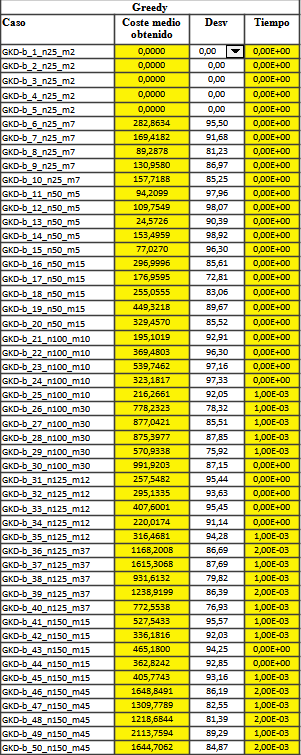
\includegraphics[width=0.3\textwidth]{tablaGreddy.png}
    \end{figure*}

    \pagebreak

    \subsubsection{Búsqueda Local}

    \begin{figure*}[h]
        \centering
        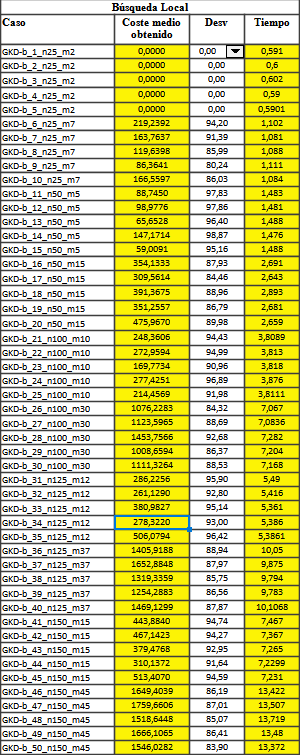
\includegraphics[width=0.3\textwidth]{tablaBL.png}
    \end{figure*}

    \pagebreak
    \subsubsection{AGG-Uniforme}

    \begin{figure*}[h]
        \centering
        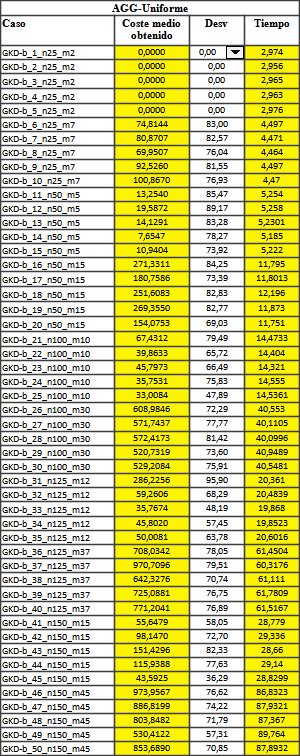
\includegraphics[width=0.3\textwidth]{tablaAGGU.png}
    \end{figure*}

    \pagebreak
    \subsubsection{AGG-Posicion}

    \begin{figure*}[h]
        \centering
        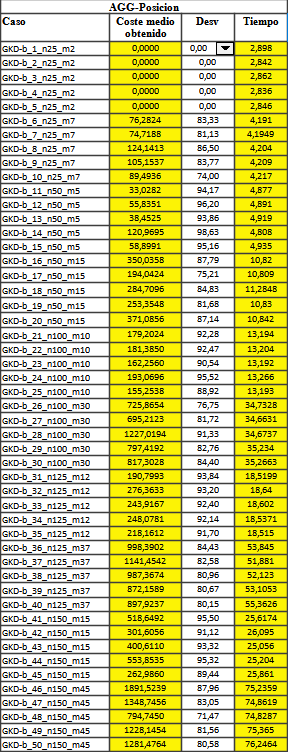
\includegraphics[width=0.3\textwidth]{tablaAGGP.png}
    \end{figure*}

    \pagebreak
    \subsubsection{AGE-Uniforme}

    \begin{figure*}[h]
        \centering
        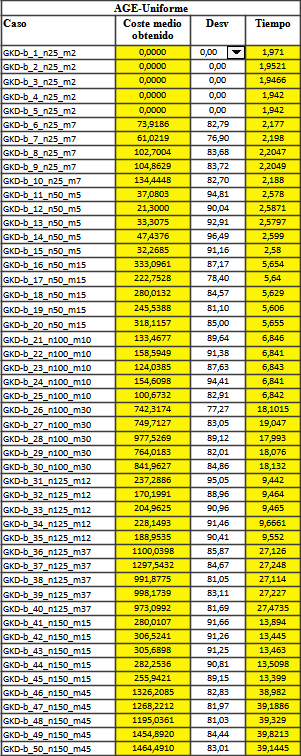
\includegraphics[width=0.3\textwidth]{tablaAGEU.png}
    \end{figure*}

    \pagebreak
    \subsubsection{AGE-Posición}

    \begin{figure*}[h]
        \centering
        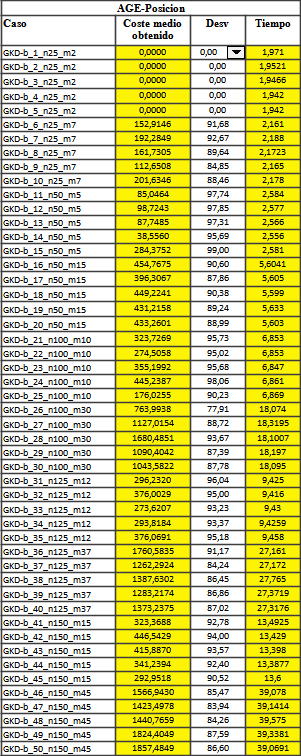
\includegraphics[width=0.3\textwidth]{tablaAGEP.png}
    \end{figure*}

    \pagebreak
    \subsubsection{Medias}

    \begin{figure*}[h]
    \centering
    \begin{tabular}{ |c|c|c| }
        \hline
        \textbf{Algoritmo} & \textbf{Desviación} & \textbf{Tiempo (s)} \\
        \hline
        Greedy             & $80.18$             & $4.8 \cdot 10^{-4}$ \\
        \hline
        BL                 & $81.58$             & $5.3$               \\
        \hline
        AGG-Uniforme       & $66.24$             & $20.78$             \\
        \hline
        AGG-Posición       & $78.43$             & $24.4$              \\
        \hline
        AGE-Uniforme       & $77.89$             & $12.7$              \\
        \hline
        AGE-Posición       & $81.84$             & $12.7$              \\
        \hline
    \end{tabular}
\end{figure*}

    \subsection{Gráficas}

    \subsubsection{Greedy}

    \begin{figure*}[h]
        \centering
        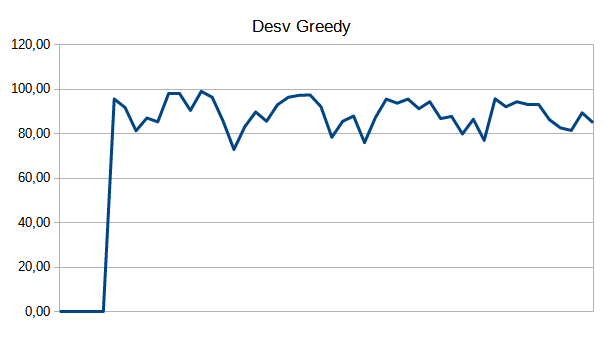
\includegraphics[width=\textwidth]{greedy.png}
    \end{figure*}

    \pagebreak
    \subsubsection{Búsqueda Local}

    \begin{figure*}[h]
        \centering
        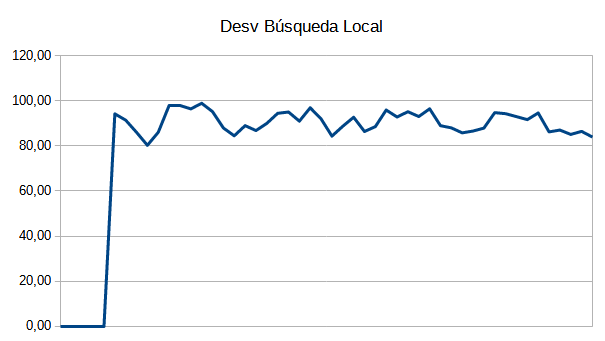
\includegraphics[width=0.85\textwidth]{desvbl.png}
    \end{figure*}

    \begin{figure*}[h]
        \centering
        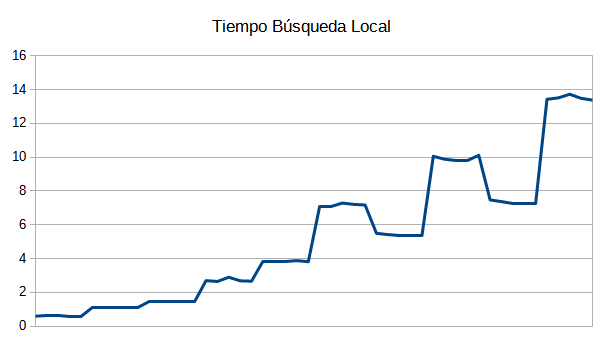
\includegraphics[width=0.85\textwidth]{tiempobl.png}
    \end{figure*}

    \pagebreak
    \subsubsection{AGG-Uniforme}

    \begin{figure*}[h]
        \centering
        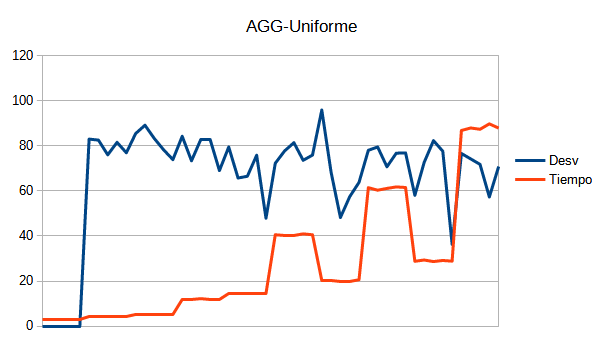
\includegraphics[width=0.85\textwidth]{graficoAGGU.png}
    \end{figure*}

    \subsubsection{AGG-Posición}

    \begin{figure*}[h]
        \centering
        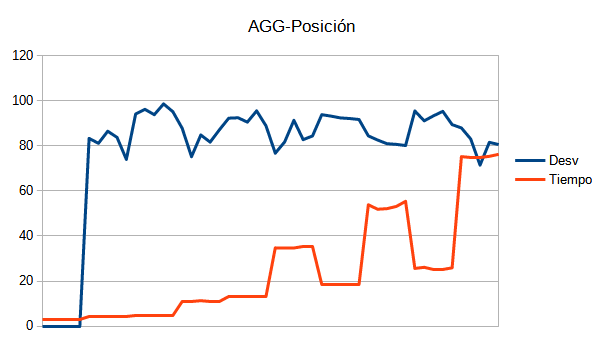
\includegraphics[width=0.85\textwidth]{graficoAGGP.png}
    \end{figure*}

    \pagebreak
    \subsubsection{AGE-Uniforme}

    \begin{figure*}[h]
        \centering
        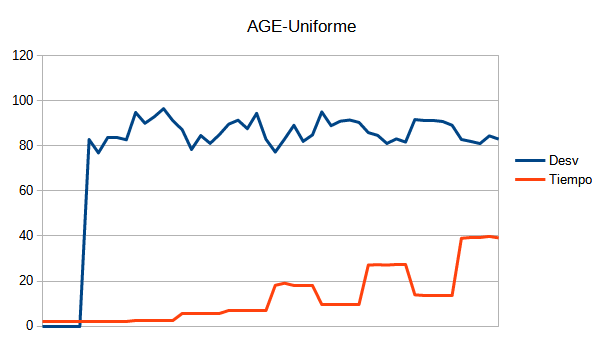
\includegraphics[width=0.85\textwidth]{graficoAGEU.png}
    \end{figure*}

    \subsubsection{AGE-Posición}

    \begin{figure*}[h]
        \centering
        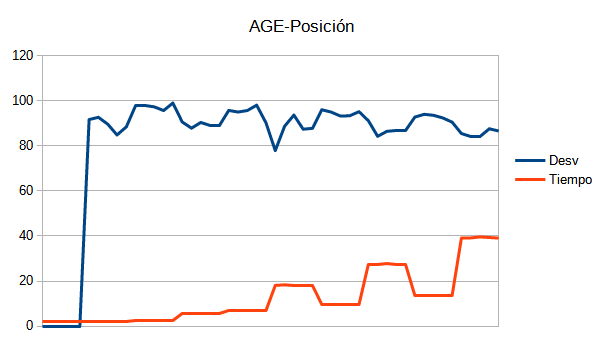
\includegraphics[width=0.85\textwidth]{graficoAGEP.png}
    \end{figure*}

    \pagebreak
    \subsection{Análisis}

    \emph{Por desgracia, como mis resultados obtenidos son \textbf{pésimos}, haré el análisis
    solamente en base a mis resultados y a mis implementaciones. Me gustaría sacar una conclusión real,
    pero solo puedo limitarme a hacer comparaciones y mencionar posibles errores.}

    \emph{El algoritmo Greedy debería de haber dado una desviación mayor que la BL.
    Los AGE en general deberían ser mejores que los AGG al ser constantes en cuanto a mejorar, además, sus tiempos son prácticamente idénticos.
    Podría decir que si puede notarse la diferencia entre el cruce uniforme y el de posición,
    pero poco.
    }

    \emph{¿Cómo puede ser que haya implementado peor el AGE-Posición que la BL?}

    \emph{En los AGG, a partir del caso 25, los tiempos empiezan a dispararse,
    llegando a superar el minuto por caso (esto se nota mucho cuando $m$ es grande)}

    \emph{Si dieran buenos resultados tendría un pase, pero a ojo,
    la desviación media de todos los algoritmos es $\approx 80$, que es demasiado. Esto es igual solamente para los genéticos.
    El que mejor lo hace de todos es el AGG-Uniforme (en un caso, puede que el 35, bajó del $40$ de desviación)}

    \emph{Lo único que hacen bien todos los algoritmos es en hacer bien los primeros 5 casos.}

\end{document}